\textnormal{
}

%\begin{itemize} 
%\item{ }
%A brief textual description of the overall flow diagram (along with its functional operation in the different user scenarios described in the first stage of the project).
%\item{ }
%A specification of each algorithm and associated data structures together with its entities, attributes, and operations ( include an English description of how they relate to your user scenario(s)).

%\end{itemize}
\begin{itemize} 
\item{  System Flow description:}  
\textnormal{The visualization of BDA* Algorithm is achieved through a GUI. The GUI opens a window in which there is a blank space provided to draw the desired graph. The user can draw vertices, edges, source and goal nodes. The user then assigns weights and heuristic values.  Once the graph has been drafted, the user may click on the confirm button to indicate that the graph has been finalized. The program then checks for validity of graph. If the graph is valid, the BDA* algorithm is implemented and the user will be shown step by step advancement of the path from the source to goal. The constraints for the validity of graph are discussed later in the document. The system and algorithmic flow diagrams are shown below.  }

\item{ Flow Diagram. }

    \begin{figure}[!h]
     \centering
      \begin{subfigure}{}
      
        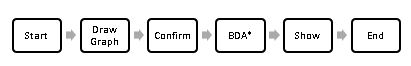
\includegraphics[width=0.5\textwidth]{system.JPG}
        \caption{System Flow}
        \label{fig:1}
      \end{subfigure}
      %
      \begin{subfigure}{}
        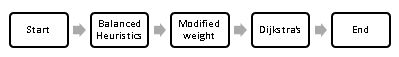
\includegraphics[width=0.5\textwidth]{algorithm.JPG}
        \caption{Algorithm Flow}
        \label{fig:2}
      \end{subfigure}
    \end{figure}

\pagebreak
\item{ High Level Pseudo Code System Description:}

\begin{lstlisting}[breaklines=true, frame=single]
def system(): #the whole system loop
    while True:
        get a new message msg from message queue
        if msg is closeMsg:
            return
        else if msg is editPaintMsg:
            disable BDA* button
            continuousStepFlag = False
            use paintBoard function to process msg
            send a new message updateMsg
        else if msg is confirmMsg:
            use confirm function to check the graph
            if graph is valid:
                enable BDA* button
        else if msg is BDASMsg:
            use preprocess function on G to prepare for BDA* searching loop
            send a new message stepMsg
        else if msg is stepMsg:
            use step function to process 1 step of BDA*
            send a new message updateMsg
            if 2 searching parts meet:
                continuousStepFlag = False
                send a new message postprocessMsg
            else if at least 1 searching part cannot continue:
                continuousStepFlag = False
            else:
                continuousStepFlag = True
        else if msg is updateMsg:
            use updatePaint function to show the graph
            if continuousStepFlag is True
                send a new message step
        else if msg is postprocessMsg:
            use postprocess to trace the path 
            send a new message updateMsg
    return

def paintBoard(msg): #paint graph
    if msg is newV:
        check if there is already a vertex at the click position
        if there is:
            report error to users
        else:
            creat a new vertex and edit it
    if msg is newE:
        check if there are already 2 vertices at 2 ends of drag
        if there are not:
            report error to users
        else:
            creat a new edge and edit it
    if msg is editV:
        check if there is already a vertex at the click position
        if there is not:
            report error to users
        else:
            find that vertex and edit it
    if msg is editE:
        check if there are already 2 vertices at 2 ends of drag
        if there are not:
            report error to users
        else:
            find that edge and edit it
    if msg is deleteV:
        check if there is already a vertex at the click position
        if there is not:
            report error to users
        else:
            find that vertex, delete it and delete all edges of it
    if msg is deleteE:
        check if there are already 2 vertices at 2 ends of drag
        if there are not:
            report error to users
        else:
            find that edge and delete it
    return



def confirm(G): #check if G is valid or not
    if there is not a start vertex:
        report error to users
        return False
    if there is not a goal vertex:
        report error to users
        return False
    use dijkstra's to compute the real distance of each vertex from start vertex

    if goal vertex is not reachable:
        report warn to users
        return True
    use dijkstra's on the reversed graph to compute the real distance of each vertex from goal vertex

    for each vertex of the graph:
        if the real distance is less than potential:
            report warn to users
    return True

def preprocess(G): #preprocess of BDA*
    for each vertex v of the graph:
        compute balanced potential
    for each edge of the graph:
        compute modified weight using balanced potential
    initialize searching
    return

def step(G): #BDA* loop
    if any priority queue is empty:
        return False
    update distance and previous vertex simultaneously from start vertex and goal vertex for one step

    if they meet at some vertex:
        return meeting vertex
    else:
        return None

def postprocess(G): #generate path and maybe preprocess for optimal path
    from meeting vertex, use previous vertex to trace the path to goal vertex and start vertex, and combine them
    return


def updatePaint(G):
    paint all vertives and edges of the graph
    highlighting the visited vertices and returned path
    return
\end{lstlisting}

\item{Algorithms and  Data Structures. }
\begin{itemize}
    \item Algorithm:

BDA* Algorithm: The BDA* algorithm implements A* algorithm from both ends of a graph simultaneously. One A* algorithm is implemented from the start node towards goal node and the other A* algorithm is implemented from the goal node towards the start node. Each vertex is given two values of heuristic, one from start node and one from the goal node. The algorithm calculates normalized weights using the heuristic values of corresponding vertices for each edge using the formula:
\[h(u) = \frac{h_s(u)-h_g(u)}{2} \]
\[w_{new}=w_{old}-(h(u)-h(v))\]
The algorithm calculates two normalized weights for each edge, one for forward A* and another for backward A*. Using these normalized weights, A* is applied in both directions and the path from the start node to goal node is found when these two converge to the same point in the graph. 

\item Data Structures:
\begin{enumerate}

    \item Python Dictionary: The python dictionary stores data in a similar way as the regular dictionary. It has keys which are associated with corresponding values and these values can be referenced using the keys.
    \item Priority Queue: A priority queue is stored in form of array/list and implemented using heaps. New values are inserted at the back and removal of values is done from the front. However, the priority of the elements is always maintained at the front and the element with the lowest priority is moved to the back.
\end{enumerate}


\end{itemize}



\item{ Constraints: }
The visualization project does not use a database for storing values. Therefore, there are no integrity constraints applicable to the project. However, there are a few algorithmic constraints to drawing a graph as follows: 
\begin{itemize}
    \item If there are no weights specified by the user, then the default value of the edge weight is 1.
    \item  If the start node or the goal node is not specified by the user, then an error is displayed prompting user to enter either or both of the start node and goal node.
    \item  If the path from the start node to goal node doesn't exist, then a warning is displayed prompting the user that no path exists.
    \item  If the heuristic is not admissive, then prompt the user warning that heuristic might not yield the best path. The user then decides whether he wants to enter heuristic values again or continue anyway.
    \item Each edge must have two existing vertices as its ends. And there cannot be an edge from u to u. 
    \item Each vertex must be at distinct positions. 
    \item Each edge must have a distinct vertex pair as its identification. There cannot be two edges from u to v.
\end{itemize}

\end{itemize}
}
